% -*- mode: LaTex; outline-regexp: "\\\\section\\|\\\\subsection";fill-column: 80; -*-
\documentclass[12pt]{article}
\usepackage[longnamesfirst]{natbib}
\usepackage[usenames]{color}
\usepackage{graphicx}  % Macintosh pdf files for figures
\usepackage{bbm}       % one symbol
\usepackage{amssymb}   % Real number symbol {\Bbb R}
\input{../../standard}

% --- margins
\usepackage{../../sty/simplemargins}
\setleftmargin{1in}   % 1 inch is NSF legal minimum
\setrightmargin{1in}  % 1 inch is NSF legal minimum
\settopmargin{1in}    % 1 inch is NSF legal minimum
\setbottommargin{1in} % 1 inch is NSF legal minimum

% --- Paragraph split, indents
\setlength{\parskip}{0.00in}
\setlength{\parindent}{0in}

% --- Line spacing
\renewcommand{\baselinestretch}{1.3}

% --- Margins
\setlength{\topmargin}{-0.5in}
\setlength{\oddsidemargin}{-0.1in}
\setlength{\textheight}{9.0in}
\setlength{\textwidth}{6.5in}

% --- page numbers
\pagestyle{empty}  % so no page numbers

% --- Hypthenation
\sloppy  % fewer hyphenated
\hyphenation{stan-dard}
\hyphenation{among}

% --- Customized commands, abbreviations
\newcommand{\TIT}{{\it  {\tiny Risk of sequential tests (\today)}}}

\newcommand{\test}{\mbox{$\hat\mu(\al(\cdot),w_0,\omega)$}}
\newcommand{\uTest}{\mbox{$\hat\mu(\al_u(\cdot),w_0,\omega)$}}
\newcommand{\gTest}[1]{\mbox{$\hat\mu(\al_g(\cdot,{#1}),w_0,\omega)$}}

% --- Header
\pagestyle{myheadings}
\markright{\TIT}

% --- Title

\title{ Risk of Sequential Testing with Alpha Investing }
\author{
        Dean P. Foster and Robert A. Stine
        \thanks{Research supported by NSF grant DMS-1106743 }  \\
        Department of Statistics            \\
        The Wharton School of the University of Pennsylvania \\
        Philadelphia, PA 19104-6340                          \\
        www-stat.wharton.upenn.edu/$\sim$stine 
}

\date{\today}


%%%%%%%%%%%%%%%%%%%%%%%%%%%%%%%%%%%%%%%%%%%%%%%%%%%%%%%%%%%%%%%%%%%%%%%%%%%

\begin{document}
\maketitle 
%------------------------------------------------------------------------

\abstract{ 

 Streaming feature selection evaluates potential explanatory variables
 sequentially rather than all at once.  This approach produces novel challenges
 for variable selection.  Spending rules such as alpha investing control the
 rate of false discoveries, but little is known about the risk of the resulting
 estimator.  We provide here a computational framework for finding and comparing
 the finite-sample, worst-case risk of streaming selection.  Our findings
 demonstrate that in all but very sparse models, estimators allowed to have
 larger rates of false discoveries produce smaller risk.  

}

%------------------------------------------------------------------------
\vspace{0.05in}

\noindent
{\it Key Phrases: Bellman equations, hard thresholding, streaming feature
 selection, testimator, variable selection}

\clearpage


% ----------------------------------------------------------------------
\section{ Introduction }
% ----------------------------------------------------------------------


 Streaming feature selection constructs a predictive model by choosing
 explanatory variables from a sequence offered by an exogenous source.  Rather
 than evaluate these variables simultaneously, streaming selection evalutes them
 one-at-a-time.  Greedy searches like stepwise regression consider the full
 batch of, say, $p$ potential explanatory variables together, choosing at the
 first step the predictor $X_{(1)}$ that obtains the best fitting model.  In
 contrast, streaming selection evaluates the offered predictors sequentially as
 $X_1, \, X_2, \ldots$, performing the evalation of $X_j$ in the context of the
 model produced by picking from $X_1, \ldots, X_{j-1}$.  Hence, streaming
 selection does not require the full set of explanatory variables at the start
 of the search and is free to use the results of evaluating initial variables to
 guide the search for those to add subsequently.  For example, if it adds $X_j$
 to the model, the streaming search might then be expand add interactions $X_j
 \, X_k$ to the queue of possible variables to consider.  Streaming selection
 can thus rapidly explore collections of explanatory variables that are larger
 than typically considered with conventional methods; the slowest step in
 forward stepwise regression is the calculation of the $X'X$ matrix.
  \citet{fosterlin10} show examples selecting from up to $p$=100,000 explanatory
 variables.


 Streaming selection poses a challenge, however, for variable selection.
  Although it is advantageous to avoid simultaneously evaluating every
 predictor, the absence of a fixed set of features in streaming selection
 requires a different type of selection criterion from those commonly used.  For
 example, suppose the search begins with a list of $p$ possible features $X_1,
 X_2, \ldots, X_p$.  As mentioned previously, the search could expand to include
 interactions in $X_j$ once $X_j$ joins the model.  If the search is limited to
 second-order interactions (one could allow higher order interactions as well),
 then the maximum number of possible explanatory variables is $m = p(p+1)/2$
 variables.  Since few of these would be considered, it would be very
 conservative to combine $m$ with a criterion such as AIC, BIC, or RIC.
  Similarly, selection using FDR requires the full set of marginal $p$-values.


 Alpha investing \citep{fosterstine08} is a sequential testing procedure
 designed to support streaming feature selection.  Because alpha investing can
 test an infinite sequence of hypotheses, it is well-matched to a search of an
 unbounded collection of features that is too large to manipulate
 simultaneously.  Rather than test multiple hypotheses at once, alpha investing
 tests hypotheses one-at-a-time in a specified order.  Alpha investing begins
 with an initial allowance for Type I error that is called its alpha wealth.
  Each test consumes some of the available alpha wealth, as in the alpha
 spending rules used in clinical trials.  Alpha investing differs from these and
 overcomes the conservatism of alpha spending rules, which include the
 Bonferroni method, by earning a contribution to the alpha wealth available for
 subsequent tests for each rejected null hypothesis.  Thus rejections beget more
 rejections.  Alpha investing further allows one to test an infinite stream of
 hypotheses, accommodate dependent tests, and incorporate domain knowledge.
 

 Though flexible, alpha investing controls the expected number of false
 rejections.  Controlling the false discovery rate with alpha investing guards
 against overfitting in variable selection.  With alpha inveseting, one can
 guarantee that on average not more than, say, 5\% of the rejected hypotheses
 spuriously add a predictor to the model.  When building a predictive model,
 however, controlling the false discovery rate is frequently secondary to
 obtaining a more predictive model.  Control of the false discovery rate does
 not imply that one will find the most predictive model possible.  It only
 guarantees that a high percentage of chosen features are in fact useful.  The
 risk of the implied estimator is more relevant.


 Our analysis here considers the cumulative risk of a sequence of testimators
 implied by testing a sequence of null hypotheses.  A testimator is also known
 as a keep-or-kill estimator or a hard thresholding estimator.  The estimator of
 a parameter $\mu$ is zero unless a test of the null hypothesis that claims $\mu
 = 0$ is rejected.  The estimation problem we consider is a simplified version
 of the variable selection problem that avoids issues related to the
 collinearities among the explanatory variables.  
 Rather than observe a sequence
 of slope estimates, we assume that the observed data are a finite sequence of
 $p$ random variables $Y_j \sim N(\mu_j,1)$.  


 \ras{ Revise roadmap paragraph }
 The following section describes the use of alpha-investing for setting the
 levels $\al_j$ of the tests that determine the testimator $\hat\mu$.  Section 3
 describes the computations that solve a set of Bellman equations.  Our
 methodology bounds the risk of any sequential testimator.  In the spirit of
 risk inflation and oracle bounds, we compute the convex set of attainable
 risks:
 \begin{equation}
   \CC(\hat\gamma) 
      = \{(x,y): \exists \mu \mbox{ for which }
                 x=R(\tilde\mu,\mu), \, y = R(\hat\mu_{\hat\gamma},\mu)\} \;,
 \label{eq:C}
 \end{equation}
 where $\tilde\mu$ identifies an oracle estimator of $\mu$ that is defined in
 Section 3.  The boundary of $\CC$ produces exact results that are comparable to
 those obtained in asymptotic multivariate setting.  Section 4 displays the risk
 of these procedures, and we conclude with a summary and discussion of open
 issues in Section 5.


% ---------------------------------------------------------------------------
\section{ Alpha-investing }
% ---------------------------------------------------------------------------

 An alpha-investing rule \citep{fosterstine08} determines the level for testing
 $H_j$ based on its alpha wealth, a limit on the maximum level that depends on
 the results of prior tests.  The procedure is most easily described by
 explaining the first few steps.  The process begins with an initial allocation
 $w_0$ \marginpar{$w_0$} of alpha wealth.  The choice of this initial alpha
 wealth is an important aspect of our analysis of the risk of $\hat\mu$.  An
 alpha-investing rule can test $H_1$ at any level up to the total available
 alpha wealth, $0 \le \alpha_1 \le w_0$.  The level $\al_1$ is `invested' and
 cannot be used for subsequent tests.  We say that $\al_1$ is invested rather
 than spent because of the way in which the outcome of the test of $H_1$
 influences the subsequent wealth.  Let $p_1$ denote the p-value of the test of
 $H_1$.  If $p_1 \le \alpha_1$, the test rejects $H_1$.  In this case, the
 alpha-investing rule earns a contribution $\omega > 0$ \marginpar{$\omega$} to
 its alpha wealth; otherwise, the alpha wealth available to test $H_1$ falls to
 $W_1 = w_0 - \alpha_1$.  In general, the alpha wealth available for the test of
 $H_{j+1}$ is given by the stochastic process \marginpar{$W_j$}
 \begin{equation}
    W_j = W_{j-1} - \alpha_j + \omega \, I_{\{p_j < \al_j\}}, \; j = 1,\,2,\ldots,
 \label{eq:Wj}
 \end{equation}
 with the initial condition $W_0 \equiv w_0$.  Alpha investing thus resembles
 alpha spending used in clinical trials, with the key distinction that rejecting
 a hypothesis earns an additional allocation $\omega$ of alpha-wealth for
 subsequent testing.  \ras{reference to QPD and enhanced alpha investing}


 Because rejecting a null hypothesis makes it easier to reject other null
 hypotheses, it is important that alpha investing controls the rate of false
 rejections.  To this end, \citet{fosterstine08} show that alpha investing
 controls a sequential version of mFDR.  Let $D(j)$ count the number of
 hypothesis rejected in the first $j$ tests, and let $V(j) \le D(j)$ denote the
 number of {\em false} rejections through the first $j$ tests.  The sequential mFDR is
 \begin{equation}
    \mbox{mFDR}_\eta(j) = \frac{\ev V(j)}{\eta + \ev R(j)} \;, \eta > 0.
 \label{eq:mFDR}
 \end{equation}
 The similar false discovery rate is essentiallyt the expected value of the
 ratio rather than the ratio of expected values.  The constant $\eta$ in the
 denominator of mFDR avoids dividing by zero under the complete null hypothesis
 in which all $\mu_j = 0$.  If $w_0 \le \omega$, then alpha-investing rules
 control $\mbox{mFDR}_\eta(p) \le \omega$, and this result implies weak control
 of the family wide error rate.  Furthermore, the index $j$ in \eqn{eq:mFDR} is
 allowed to be an arbitrary stopping time, such as the occurrence of the $k$th
 rejection.

 
 Alpha-investing rules are quite general.  The underlying theory requires only
 that the level of the test of $H_j$ is bounded by the available wealth
 $W_{j-1}$ and that the test indeed have level $\al_j$, conditional on the
 outcomes of prior tests.  Otherwise, an alpha-investing rule is allowed to use
 the pattern of prior rejections as captured by the sequence of wealths.  We can
 capture this dependence by thinking of the investing rule ${\cal A}$ as a
 function of the sequence of prior wealths $W_0^j = \{W_0, W_1, \ldots, W_j\}$.
  A rule is then a map from the sequence of wealths to a number on the interval
 0 to the current wealth:
 \begin{equation}
    {\cal A}: W_0^j \mapsto [0, \min(W_j,1)]    
 \label{eq:A}
 \end{equation}
 For example, the rule $\cal A$ can set the wealth of the next test higher or
 lower depending upon how long since the last rejection or the number of
 rejections to this point.  Though alpha investing allows this complete
 generality, we focus our attention on a simpler class of investing rules with a
 path independent, Markovian structure.  The amount invested by these rules
 depends only on the current wealth rather than the full path, ${\cal A}(w_0^j)
 = \al(W_j)$.  The only requirement is that $0 \le \al(w) \le w$; a rule cannot
 invest more wealth than the amount possessed.  It does seem natural, however,
 for $\al(w)$ to be monotone increasing in $w$.


 The simplest representatives of this class of alpha investing rules are
 geometric rules.  These invest a fixed percentage of the available wealth on
 each test:
 \begin{equation}
    \al_g(w, \psi) = \psi \, w, \quad  0 < \psi < 1.
 \label{eq:Ageo}
 \end{equation}
 Though independent of the rejection path, geometric rules invest more heavily
 following a rejection.  Since the alpha wealth increases after a rejection, a
 geometric rule $\al_g$ invests more following a rejection and then gradually --
 depending on $\psi$ -- reduces the level of subsequent tests.


 The following investing rule varies the invested share.  Rather than investing
 a fixed share of the available wealth, it invests a progressively smaller share
 of the available wealth as the wealth drops.  The rule is defined by
 \begin{equation}
   \al_u(w) = w - \frac{\log 2}{\log(1+2^{1/w})} \;.   
 \label{eq:Auniv}
 \end{equation}
 Because this investing rule is related to the universal prior for integers
 defined by \citet{rissanen83}, we call this a universal investing rule and
 identify it by a subscript $u$.  (See the following remark.)  For very large
 wealth, $\al_u(w)$ approaches $w$ (the limit of the second term in
 \eqn{eq:Auniv} is $w-1$ as $w \rightarrow \infty$), and $\al_u(w)
 \rightarrow 0$ as $w \rightarrow 0$.

 
 Figure \ref{fig:rules} contrasts the investments produced by the universal and
 several alpha investing rules on a log-log scale.  The initial wealth for all
 rules is set to $w_0 = 1$.  With this scaling, the amounts invested by the
 universal rule falls off approximately linearly.  The amounts invested by the
 universal rule are initially larger than those of any of these geometric rules.
  With $w_0=1$, the universal rule invests about $0.369$, $0.131$, $0.0693$,
 $0.0438$, and $0.0306$ in the first five tests before its spending gradually
 slows. After this initial period, each geometric rule has a range of tests over
 which the geometric rule provides a larger alpha level for testing $H_j$ than
 the universal rule.  Ultimately, however, each geometric rule invests smaller
 amounts than the geometric rule as the testing continues.  For example, the
 geometric rule that invests 1\% of its current wealth at each test
 ($\psi=0.01$) invests more than the universal rule when testing $H_{11}$
 through $H_{581}$. \ras{ Say more here about why this 'blending' of the
 geometric rates is a good thing; too bad we don't have that 'habitation' idea
 worked out where the universal finds a steady rate appropriate for the rate of
 false nulls. }


 \begin{figure}
 \caption{ \label{fig:rules} \sl Investments for the universal and several
 geometric alpha investing rules if no intervening test rejects. }

 \centerline{
 \vspace{0.1in}
 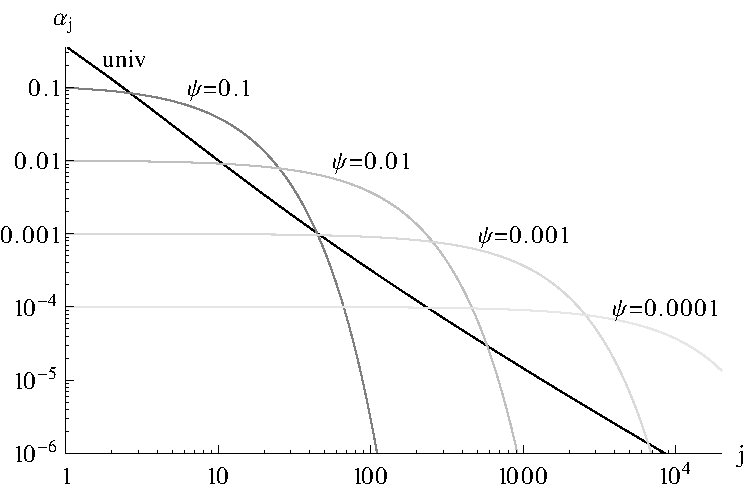
\includegraphics[width=3.5in]{figures/rules} }
 \vspace{0.2in}
 \end{figure}


 \vspace*{0.2in}
 \noindent
 {\it Remark A. }  We obtained the universal rule by the following construction
 that links a spending rule to a probabilty distribution that allocates the
 current wealth over subsequent tests.   

We illustrate the construction for the geometric rule.  If the initial wealth
 is $w_0$, then the alpha wealth invested in the $j$th test (assuming no
 intervening test rejects) is
 \begin{equation}
    \al_j = w_0\; \psi \; (1-\psi)^{j-1} \;, \quad j = 1, 2, \ldots\;.   
 \label{eq:alj1}
 \end{equation}
  Rather than define the investing rule using a discrete distribution on
 $j=1,\,2,\ldots$ as in \eqn{eq:alj1}, use the continuous density
 \begin{equation}
   A_g(x,\psi) = c_g \; \psi\,(1-\psi)^{x-1}, \quad 1 \le x\;,
 \label{eq:alg}
 \end{equation}
 where the normalizing constant $c_g = -\log (1-\psi)/\psi$.  Notice that the
 wealth invested in the $j$th test \eqn{eq:alj1} matches the integral of
 $A_g(x)$ from $x=j$ to $x=j+1$,
 \begin{equation}
    \al_j = w_0 \int_j^{j+1} A_g(x,\psi) dx = w_0 \, \psi\; (1-\psi)^{j-1} \;.
 \label{eq:alj2}
 \end{equation}
 To move away from this discrete indexing, note that the following tail integral
 shows the amount of wealth that remains,
 \begin{equation}
    W_g(x) = w_0 \int_x^\infty A_g(t,\psi) dt = w_0 (1-\psi)^{x-1}\;.
 \label{eq:Wg}
 \end{equation}
 For integers $j$, $W_g(j)$ is the wealth remaining after $j$ tests that fail to
 reject.  By inverting this tail integral, we obtain an investing rule that
 requires only the available wealth,
 \begin{equation}
   \al_g(w,\psi) = A_g(W_g^{-1}(w),\psi) = \psi\,w \;,
 \label{eq:Ag}
 \end{equation}
 as in \eqn{eq:Ageo}.  This construction uses the inverse of the tail wealth to
 determine a `test index' $W_g^{-1}(w)$ that corresponds to the current input
 wealth $w$.  The universal rule $\al_u(w)$ follows from the same
 contruction, with the density
 \begin{displaymath}
    A_u(x) = \frac{\log 2}{(x+1) (\log(x+1))^2} \;, \quad 1 < x,
 \end{displaymath}
 used in place of $A_g$.

 \vspace*{0.2in}
 \noindent
 {\it Remark B. } To avoid adding notation, we overload the symbol $\al$.  By
 itself, we use $\al$ to represent the generic level of a test.  When given an
 integer subscript, $\al_j$ is the level of the $j$th test in sequence of tests,
 as in \eqn{eq:alj1}.  Finally, when denoting a function, $\al(w)$ is the level
 invested in a test by a procedure that has available wealth $w$, as in
 \eqn{eq:Ageo} or \eqn{eq:Auniv}.  Throughout these uses, the symbol $\alpha$
 consistently gives the level of a test; only the context of the test changes.


%--------------------------------------------------------------------------
\section{ Risk Analysis}
%--------------------------------------------------------------------------

 We start by considering the risk of testimators in the case of a single test or
 multiple simultaneous tests.  This foundation allows us to introduce the
 approach that we take when studying the risk produced by alpha investing
 procedures in the sequential context.


 We first consider the squared error risk of testimators for a single parameter.
  Let $Y \sim N(0,1)$.  The scalar testimator defined by the two-sided test of
 $H_0: \mu=0$ at level $\al$ is
 \begin{equation}
   \hat\mu_\al(Y) = \left\{
     \begin{array}{cc}
        Y & \mbox{ if } z_\al^2 \le Y^2, \cr
        0 & \mbox{ otherwise, }
      \end{array} \right.
 \label{eq:muHat}
 \end{equation}
 where $z_\al$ denotes the positive, two-sided critical value
 \begin{equation}
   z_\al = \Phi^{-1}(1-\al/2) \;.
 \label{eq:zAlpha}
 \end{equation}
 The risk of $\hat\mu_\al$ is
 \begin{eqnarray}
   R(\hat\mu_\al(Y), \mu) 
     &=& \ev(\hat\mu_\al(Y) - \mu)^2  \cr
     &=& \mu^2 \pr(Y^2 \le z_\al^2) 
         + \int_{y^2>z_\al^2} (y-\mu)^2 \phi(y) dy \cr
     &=& B_\al(\mu) + V_\al(\mu)
 \label{eq:risk_mu_al}
 \end{eqnarray}
 The first summand $B_\al(\mu)$ is the squared bias that arises if the test of
 $H_0: \mu=0$ does not reject when $\mu \ne 0$; the second summand is the
 variance of the estimator.  Figure \ref{fig:risk}(a) shows a graph of the risk
 of testimators with $\al=0.05$ and $\al = 0.20$.  The maximum risk that occurs
 near $z_\al$ grows as the level $\al$ shrinks.  Figure \ref{fig:risk}(b) shows
 the decomposition of the risk of $\hat\mu_\al$ into $B_\al(\mu)$ and
 $V_\al(\mu)$ for $\al = 0.05$.  Because the variance component $V_\al(\mu)$
 increases smoothly to its maximum 1 for large $|\mu|$, it is the bias that
 produces the noticeable peak that identifies the maximum risk just outside
 $z_\al$.


 \begin{figure}
 \caption{ \label{fig:risk} \sl Risk of testimators. (a) Risk of testimators with
 $\al$ = 0.05, 0.20 versus $\mu$. (b) Squared bias and variance components of the
 risk of $\hat\mu_{0.05}$. } 
 \vspace{0.1in}
\centerline{
 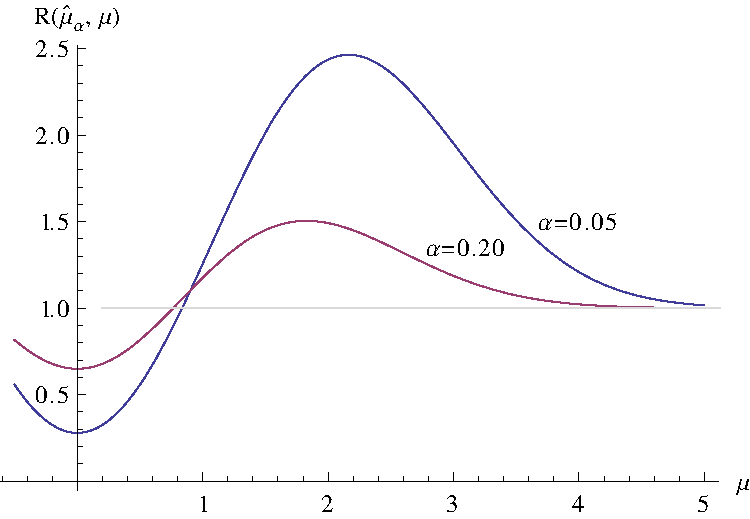
\includegraphics[width=3.0in]{figures/risk_a}
 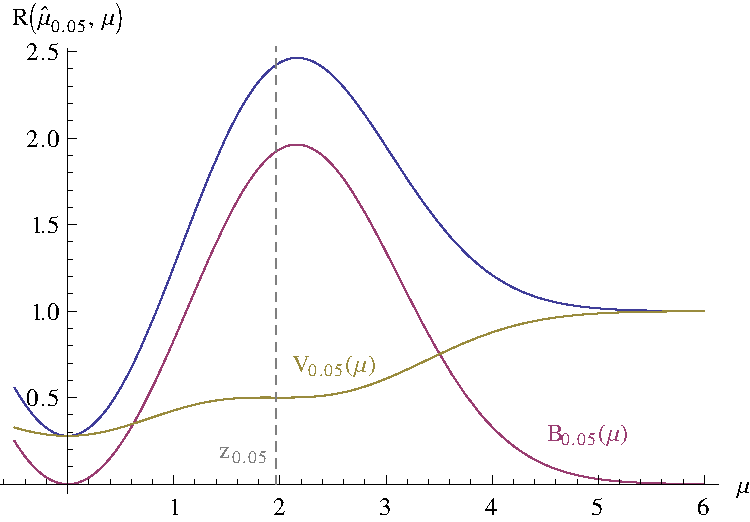
\includegraphics[width=3.0in]{figures/risk_b} }
 \vspace{0.2in}
 \end{figure}
 

 The analysis of the risk of testimators is typically done in the context of
 estimation a vector of $p$ means, $\bmu \equiv \mu_{1:p} =
 (\mu_1,\ldots,\mu_p)'$.  The available data is the vector $\YY \equiv Y_{1:p} =
 (Y_1, \ldots, Y_p)'$ with distribution $\YY \sim N(\bmu,I_p)$.  The estimator
 of $\bmu$ combines testimators at a common level in each coordinate,
 $\hat{\bmu}_\al = (\hat\mu_\al(Y_1), \ldots, \hat\mu_\al(Y_p))'$.  The estimator
 $\hat{\bmu}_\al$ consists of zeros except for those coordinates where $z_\al^2
 \le Y_j^2$.  The risk of $\hat{\bmu}_\al$ is the sum of the risks of the
 coordinate testimators,
 \begin{equation}
    R(\hat{\bmu}_\al, \bmu) 
      = \ev\; \normsq{\hat{\bmu}_\al - \bmu} \;,
 \label{eq:risk}
 \end{equation}
 where $\normsq{x} = x'x$ for vectors $x$.  We note that our notation suppresses
 the dependence of the estimator $\hat{\bmu}_\al(\YY)$ on the data.  The full
 vector $\YY$ is available for setting the level as well.


 Minimax bounds for the risk $R(\hat{\bmu}_\al,\bmu)$ are well-understood.  We briefly
 review the results of \citet{fostergeorge94} who introduced the concept of the
 risk inflation of an estimator. \citep[][obtain similar results.]
  {donohojohnstone94} The risk inflation of $\hat{\bmu}_\al$ is the supremum of
 the ratio of the risk of the testimator $\hat{\bmu}_\al$ at level $\al$ to the
 risk of a testimator that obtains the optimal level from an oracle. 
  Their results imply that the risk inflation of $\hat{\bmu}_\al$ is
 asymptotically $2 \log p$,
 \begin{equation}
    2 \log p - o(\log p) 
    \le
    \sup_\mu  \frac{1 + R(\hat{\bmu}_\al,\bmu)}
                   {1 + \inf_\eta{R(\hat{\bmu}_\eta,\bmu)}}  
    \le 
    2 \log p + 1 \;.
 \label{eq:ri}
 \end{equation}
 Foster and George further show that the testimator $\hat{\bmu}_{1/p}$ --
 essentially the Bonferoni estimator -- obtains the risk inflation threshold.
  The constant 1 added to the risks in the ratio of \eqn{eq:ri} arises in the
 context of regression models in which one always estimates the intercept.  As a
 practical device, its presence in the denominator avoids dividing by zero under
 the complete null model in which $\mu_j = 0$ for all $j$.


 Though suggestive, these results do not reveal the risk of the testimator
 derived from alpha investing.  The key difference lies in the timing of the
 choice of the test levels.  The testimator studied in risk inflation
 $\hat{\bmu}_\al$ uses a fixed level $\al$ for all $p$ coordinates, and all of
 the elements of \YY are used to set this common level.  In sequential testing,
 the $Y_j$ are observed sequentially so that the elements of the estimator form
 a stochastic process, which we collect in a $p$-element vector as
 \begin{equation}
   \hat\mu(\al(\cdot),w_0,\omega) = (\hat\mu_{\al(w_0)}, \hat\mu_{\al(W_1)}, \ldots, 
                       \hat\mu_{\al(W_{p-1})})',
 \label{eq:muHatAlphaInv}
 \end{equation}
 where $\al(\cdot)$ denotes the defining investing rule, $w_0$ is the initial
 alpha wealth, and $\omega$ is the payout earned when rejecting a hypothesis.
  The wealth random variables $W_j$ given in \eqn{eq:Wj} contribute the
 randomness.  Not only does alpha investing allow the levels to vary over the
 testimators, but the levels form a Markov process; the level of the $j$th
 testimator depends on whether prior tests reject $H_k$, $k < j$.


 The most convenient expression for the risk of \test\ relies on a recurrence.
  For convenience, let
 \begin{equation}
   r_\mu(\al) = \Phi(\mu-z_\al)+\Phi(-\mu-z_\al)   
 \label{eq:rMu}
 \end{equation}
 denote the probability of rejecting $H_0: \mu=0$ using a two-sided $z$-test at
 level $\al$ (the power of the test).  The risk of the testimator given by alpha
 investing can then be decomposed as
 \begin{eqnarray}
   R(\hat\mu(\al(\cdot),w_0),\mu_{1:p}, \omega) 
    &=& R(\hat\mu_{\al(w_0)},\mu_1)
           + \ev \sum_{j=2}^p R(\hat\mu_{\al(W_{j-1})},\mu_j)  \cr
    &=& R(\hat\mu_{\al_1},\mu_1)
           + r_{\mu_1}(\al_1)\; 
               R(\hat\mu(\al(\cdot),w_0-\al_1+\omega,\omega),\mu_{2:p})\cr
    & & \qquad + (1-r_{\mu_1}(\al_1))\; 
               R(\hat\mu(\al(\cdot),w_0-\al_1,\omega),\mu_{2:p}) \;,
 \label{eq:riskTestAI}
 \end{eqnarray}
 where $\al_1 = \al(w_0)$ and we have suppressed the dependence of the estimator
 on the data.  The second expression for the risk emphasizes the recursive
 nature of the risk and hints at our approach to its maximization using Bellman
 equations.


%--------------------------------------------------------------------------
\section{ Feasible Risk Set }
%--------------------------------------------------------------------------


 The analysis and calculation of the maximum risk obtained by the testimator
 \test\ requires a similar recursive perspective.  Suppose that the initial
 level $\al_1 = \al(w_0)=0.05$; the graph in Figure \ref{fig:risk}(b) shows the
 components of the risk of this testimator.  The choice of $\mu_1$ is not so
 simple, however, as setting $\mu_1 = \arg \max R(\hat\mu_{0.05},\mu) \approx
 \pm 2.16$.  Doing so ignores the payoff $\omega$ obtained if $H_1$ is rejected
 and its impact on the subsequent wealths $W_j$.  This choice for $\mu_1$
 maximizes the risk for the first test, but leaves a good chance for the
 estimator to gain wealth for subsequent tests by rejecting the first null
 hypothesis.  The probability that the first test rejects is
 $r_{\tilde\mu}(0.05) \approx 0.58$.  By rejecting the first test, the alpha
 investing rule obtains the additional contribution $\omega$ to its alpha
 wealth, allowing it to increase the level -- and so potentially reduce its risk
 -- in subsequent tests.  Instead, the problem to be solved at the first test is
 to choose
 \begin{eqnarray*}
    \mu_1 = \arg \max_{m} & \Bigl\{ & R(\hat\mu_{\al_1},m) \Bigr. 
        + r_{m}(\al_1) \; \max_{\mu_{2:p}} 
              R(\hat\mu(\al,w_0-\al_1+\omega,\omega),\mu_{2:p})\cr
    & & + \Bigl. (1-r_{m}(\al_1)) \max_{\mu_{2:p}} \; 
              R(\hat\mu(\al,w_0-\al_1,\omega),\mu_{2:p}) \Bigr\} \;.
 \end{eqnarray*}
 The optimal choice for $\mu_1$ depends on the risk produced by subsequent
 components of the sequence of testimators.  Notice also that the subsequent
 maximizing means are not deterministic; rather this maximization defines a
 stochastic process that maximizes on average the risk.  We identify the process
 that generates means that maximize the risk by adding braces, $\{\bmu\}$, as a
 reminder that the calculation of the risk involves a further layer of
 expectations.  


 Our interest is not just in the risk of a testimator, however, but in the
 relative risk of the testimator compared to an alternative.  In the style of
 risk inflation \eqn{eq:ri}, we want to contrast the risk of \test\ to that of a
 testimator that has no restrictions on its alpha wealth or an oracle-based
 testimator that `knows' $\mu$.  The oracle-based testimator has elements
 \begin{equation}
   \tilde\mu_j(Y_j) = \left\{ \begin{array}{cc} 
                       0    & \mbox{ if } \mu_j^2 \le 1,        \cr
                       Y_j  & \mbox{ otherwise. }
                \end{array} \right.
 \label{eq:muTilde}
 \end{equation}
 so that its risk is 
 \begin{equation}
    R(\tilde{\bmu},\bmu) = \sum_j \min(\mu_j^2,1) \;.   
 \label{eq:riskMuTilde}
 \end{equation}


 We use a feasible set to summarize the comparison of the risk of two estimators
 in the context of sequential tests.  Let $\hat{\bmu}_1$ and $\hat{\bmu}_2$
 denote two estimators for the mean vector $\mu_{1:p}$.  The feasible risk set
 for two estimators is defined as
 \begin{equation}
     {\cal R}_p(\hat{\bmu}_1,\hat{\bmu}_2) = 
      \{(x_1,x_2): \exists \{\bmu\} \mbox{ s.t. }
          x_1 = \evsub{\{\bmu\}} R(\hat{\bmu}_1,\bmu),
          x_2 = \evsub{\{\bmu\}} R(\hat{\bmu}_2,\bmu)  \} \;.           
 \label{eq:feasibleSet}
 \end{equation}
 In words, a point $(x,y)$ lies in the feasible set ${\cal R}_p$ if there exists
 a mean process $\{\bmu\}$ of length $p$ for which the expected value with
 respect to the mean process of the risk of $\hat{\bmu}_1$ is $x$ and the
 expected risk of $\hat{\bmu}_2$ is $y$.  A simple randomization argument proves
 that the feasible set must be convex.  If $x$ and $y$ are two points within
 ${\cal R}$, then there exist stochastic processes $\{\bmu\}_x$ and
 $\{\bmu\}_y$, say, that produce these risks.  The risk produced by the
 randomized process that picks $\{\bmu\}_x$ with probability $0 \le a \le 1$ and
 picks process $\{\bmu\}_y$ with probability $1-a$ is then $a\,x+(1-a)\,y$.


 Figure \ref{fig:riFeasibleSet} shows two views of the the feasible set for the
 oracle testimator versus the universal testimator \uTest\ defined by the wealth
 function $\al_u(\cdot)$ defined in \eqn{eq:Auniv}.  For this figure $p$=1,000
 tests and the initial wealth and payout $w_0 = \omega = 0.5$.  The risk of the
 oracle testimator define the x-axis and those of the universal testimator lie
 on the y-axis.  The feasible risk set is the shaded region in each frame.  The
 frame on the left of Figure \ref{fig:riFeasibleSet} shows the feasible set on
 the scale of risks; the frame on the right shows the same data on log scales.
  (The feasible risk set is not convex on a log scale but the approximation is
 quite close in practice.) To graph the risk on the log-log scale, we added 1 to
 the risks of both estimators, in the fashion of risk inflation, in order to be
 able to show the feasible risk set near 0 on a log-log scale.  Points along the
 boundary of the feasible set identify the locations at which we computed the
 risks using the method described in the following section.  The entire feasible
 set lies above the diagonal; by construction, no testimator can have smaller
 risk than obtained by this oracle estimator.  The plot on the risk scale
 emphasizes the performance in models with substantial signal; the risk of the
 oracle reaches $p$ in the saturated model in which every $1 < \mu_i$.  The plot
 on the log scale emphasizes sparse models, the so-called nearly black context
 in which most $\mu_i = 0$.  In this frame, the line parallel to and above the
 diagonal is the risk-inflation boundary that obtains for non-sequential
 estimators.  The bounds in \eqn{eq:ri} imply that the worst case risk for the
 testimator should be about $1 + 2 \log p$ times the risk of the oracle.  These
 calculations show that the risk of \uTest\ does indeed fall below this
 boundary.  \ras{ Say more about the cool shape of the risk as the risk of the
 oracle goes to zero? }


 \begin{figure}
 \caption{ \label{fig:riFeasibleSet} \sl Feasible set comparing the risk
 inflation oracle to the risk of the universal estimator \uTest with
 $w_0=\omega=0.5$ with $p$=1,000 tests on the scale of risks (left) or log risks
 (right).  Curves within the feasible set show the risks for varying signal
 levels defined in \eqn{eq:muj}}

 \vspace{0.1in}
\centerline{
 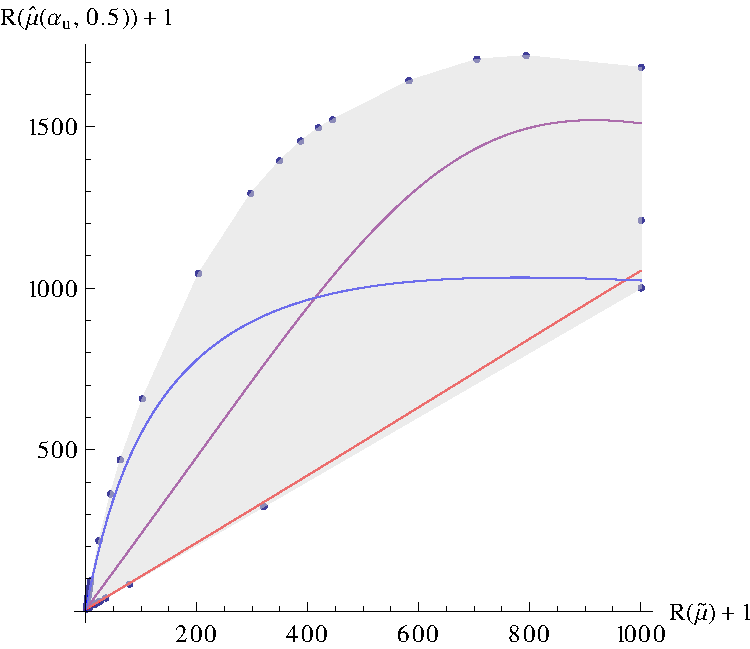
\includegraphics[width=3.0in]{figures/riFeasSet}
 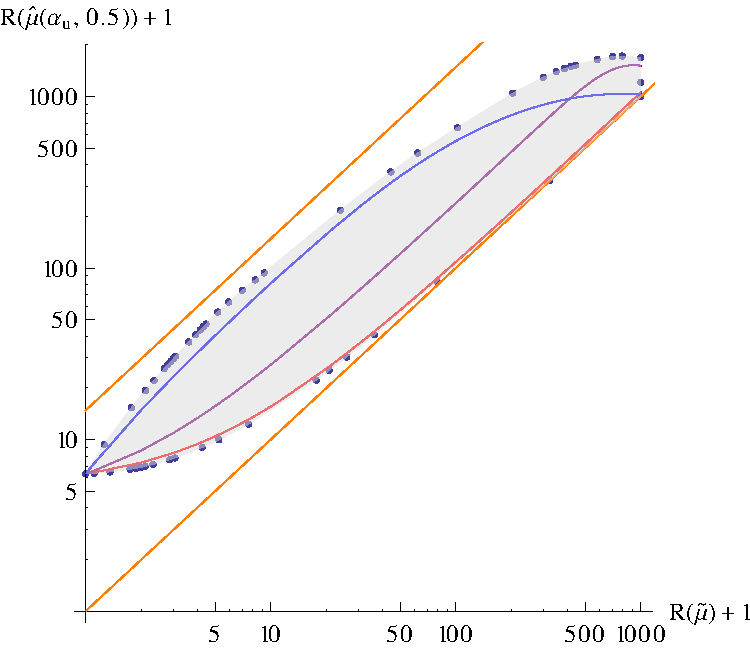
\includegraphics[width=3.0in]{figures/riFeasSetLog} }
 \vspace{0.2in}
 \end{figure}


 Curves within the feasible set show the risks of the two testimators that
 results if the means $\mu_{1:p}$ are determined by a two-point Bayesian model.
  Suppose that the stochastic process $\{\bmu\}$ that determines the means sets
 $\mu_j$ at random to some non-zero value $\mu^{*}$:
 \begin{equation}
    \mu_j = B_j \; \mu^{*}, \quad B_j  \iid \mbox{ Bernoulli}(\pi)  \;.
 \label{eq:muj}
 \end{equation}
 The smooth curves within the feasible set show the risks under this
 probabilistic model, with $\mu^{*}$ = 1.0 (red), 1.5 (magenta), or 3 (blue),
 and the probability of a non-zero mean varying over the range $10^{-6} \le \pi
 \le 1-10^{-6}$.  With $\mu^{*} = 1.0$, the risks nearly trace out the lower
 boundary of the feasible set. 



 \ras{ Talk about simulating the mean processes; or save for another day? }





%--------------------------------------------------------------------------
\section{ Computation }
%--------------------------------------------------------------------------


  Because the risk-inflation estimator $\tilde{\bmu}$ has no wealth constraint,
 we describe first the calculation of the feasible set ${\cal R}_p(\hat\mu(
 \al(\cdot), w_0, \omega), \tilde{\bmu})$.  For convenience, we abbreviate the
 alpha investing estimator as $\hat{\bmu}$ with the understanding that it
 depends on the choice of the investing function $\al(\cdot)$, $w_0$, and
 $\omega$ throughout this section.  The feasible set is two-dimensional, so we
 simplify the optimization task by finding the maximum of a mixture of the
 risks.  Let
 \begin{equation}
   U_\theta(\{\bmu\}) = \ev_\mu 
       \cos(\theta) R(\hat{\bmu}, \bmu) + \sin(\theta) R(\tilde{\bmu},\bmu) 
 \label{eq:bTheta}
 \end{equation}
 for some $ 0 \le \theta \le 2 \pi$.  The maximum utility defines a point on the
boundary of the feasible set,
 \begin{equation}
   b(\theta) = \max_{\{\bmu\}} U_\theta(\{\bmu\})  \;.
 \label{eq:bTheta}
 \end{equation}
 If we let $\{\bmu\}_\theta$ denote the stochastic mean process that maximizes
 $b(\theta)$, then the point $(R(\hat{\bmu}, \bmu), R(\tilde{\bmu}, \bmu))$ lies
 of the boundary of ${\cal R}_p(\hat{\bmu},\tilde{\bmu})$.  These are the points
 shown in plots of the feasible set, such as Figure \ref{fig:riFeasibleSet}.  By
 varying $\theta$ over the circle, we identify the feasible set as the
 intersection of the resulting half-planes.

 
 We solve the maximization \eqn{eq:bTheta} via backward induction.  The
 calculation begins with preliminary steps that build a data structure that
 tracks the wealth of the alpha investing estimator.  Building this structure
 requires identifying a grid of wealths $g$ and a jump table that caches indices
 that speed later calculations.  The wealth grid spans the minimal attainable
 wealth ($w_0 - \sum_{j=1}^p \al_j$) to a maximum allowed wealth, which we set
 to $w_{\max} = 5$.  (Our results have not been sensitive to the choice so long
 as it is substantially larger than $w_0 + \omega$.)  The wealth grid is
 `logarithmically' spaced, with a finer grid at spaced at increments 0.001 for
 small wealths below 0.02 and gradually increased.  The number of elements in
 the wealth grid determines the number of columns in a matrix $M$ that holds the
 intermediate wealths when solving the Bellman equation; the rows in this matrix
 identify the specific test.  During the calculations, $M_{jk}$ holds the
expected risk after the test of $H_j$ for an estimator with wealth $g_k$
 associated with $\hat{\bmu}$ in row $j$ of $M$ refer to the test of
 $H_j$, and a final extra row $M_{p+1,\cdot}$ defines the initial conditions for
 the recursion. (The full matrix $M$ is not necessary, but its use simplifies the
 description of the algorithm.)


 This set is more easy to find than others
 because the The wealths of the investing rules induction

a backward induction \begin{eqnarray*}
    \mu_1 = \arg \max_{m} & \Bigl\{ & R(\hat\mu_{\al_1},m) \Bigr. 
        + r_{m}(\al_1) \; \max_{\mu_{2:p}} 
              R(\hat\mu(\al,w_0-\al_1+\omega,\omega),\mu_{2:p})\cr
    & & + \Bigl. (1-r_{m}(\al_1)) \max_{\mu_{2:p}} \; 
              R(\hat\mu(\al,w_0-\al_1,\omega),\mu_{2:p}) \Bigr\} \;.
 \end{eqnarray*}


 
 Now consider the general case of the test of $H_j$.  Assume that the alpha
 wealth available to the two investing rules is $A_j$ and $B_j$, respectively,
 at this stage, and that it has been $\ell \le j$ tests since the last rejection
 by the first rule and $m \le j$ tests since the last rejection by the second.
  Assume also for ease of presentation that the level $\al_j = A_j f(\ell)$
 invested in the test of $H_j$ by the first investing rule is less than the
 level $\beta_j = B_j g(m)$ invested by the second ($\al_j < \beta_j$). It
 follows that, when utility is measured by the number of rejections, that we
only need a one-dimensional optimization at each test,
 \begin{eqnarray}
   C^\gamma_j(A_j,\ell;B_j,m) 
    &=& \max_{\mu \in \R } \left[ r^{}_{\mu}(\al_j) - \gamma \, r_{\mu}(\beta_j)\right. \cr
    && \;+ \quad r_{\mu}(\al_j) \qquad \quad
              C^\gamma_{j+1}(A_j+\omega-\alpha_j,0;\,B_j+\omega-\beta_j,0)  \cr
    && \;+ (r_\mu(\beta_j)-r_\mu(\al_j)) \; 
              C_{j+1}^\gamma(A_j-\alpha_j,\ell+1;\,B_j+\omega-\beta_j,0) \cr
    && \;+ \left.  (1-r_\mu(\beta_j)) \; 
              C_{j+1}^\gamma(A_j-\alpha_j,\ell+1;\,B_j-\beta_j,m+1) \right] \;,
 \label{eq:util}
 \end{eqnarray}
 with the boundary condition $C_{T+1}^\gamma = 0$.  The successive lines
 identify the expected differential in the number of rejections produced by the
 test of $H_j$, and following summands denote the subsequent expected values if
 both reject, if only the rule with the larger alpha level rejects, and if
 neither rejects.  


 Practical solution of the recursion for $C_1^\gamma$ requires a discrete
 approximation.  Notice in \eqn{eq:util} that the state of the recursion depends
 on the wealths of the two investing rules. Feasible calculation requires that
 we restrict the possible wealths to a discrete grid.  If the wealths are
 allowed to vary over any $W \ge 0$, then solving this recursion for any sizable
 $T$ is intractable.  Our approach discretizes the wealth functions so that the
 optimization occurs over a grid for each test $j$ rather than the positive
 quadrant of $\R^2$.  For each investing rule, we initialize a grid of $T+M+1$
 wealth values $w_j$, indexed from $j=M, M-1, \ldots, 1, 0, -1, \ldots, -T+1,
 -T$.  This grid holds the state of the wealth at each test, and the differences
 in adjacent wealths determine the amounts used to test the next hypothesis.
  For the rule defined by the distribution $f \in {\cal F}$, we set $w_0 = W_1$,
 $w_{-1} = w_0(1-f(0))$, $w_{-2} = w_{-1}(1-f(1)), \ldots$.  If the investing
 rule does not reject any hypotheses, these wealths are exact.  If the rule does
 reject, we accumulate the utility as though performing a randomized test that
 tosses a biased coin to decide which of the nearby wealths to spend.  Suppose
 that the alpha wealth when rejecting is $X = w_j + \omega$.  It is unlikely
 that $X$ lies at one of the grid of wealth values, so assume that $x = c \, w_k
 + (1-c) w_{k+1}$ for some $0 < c < 1$.  In this case, we treat the next test as
 a randomized test.  The test earns the expected utility from wealth $w_k$ with
 probability $(1-c)$ and from wealth $w_{k+1}$ with probability $c$. Basically,
 this approximation adds a second expectation to the sum in \eqn{eq:util}. We
 set $w_j$ for $j > 0$ somewhat arbitrarily in a manner that prevents the
 accumulation of excess wealth.  In our examples, $M=5$ with $w_i = W_1 + i
 \,\omega/3$, $i=1,2,3$, and $w_i = w_{i-1} + \omega$ for $i=4,\,5$.  Should the
 wealth reach $w_4$, then the bid for the next test is $\omega$, the amount
 earned by a rejection.  Hence, the testing does not increment the wealth beyond
 this boundary.
 

 We obtain a performance envelope by varying the competitive factor $\gamma$.
  To find the boundary points below the diagonal, we reverse the roles of the
 alpha investing rules and repeat the optimization.  As the optimization
 proceeds, we accumulate the component utilities that identify the boundary
 point.


%--------------------------------------------------------------------------
\section{ Examples }
%--------------------------------------------------------------------------
 
 The examples in this section compute the feasible risks produced by the alpha
 investing rules just described.  We also consider several choice for the payoff
 $\omega$ that controls mFDR.  The choices span from the conventional Type I
 error rate with $\omega=0.05$ to $\omega = 0.5$ and larger.  Setting
 $\omega=0.5$ implies that we allow up to half of the rejected hypotheses to be
 Type I errors.  Such a large error rate would not be used in testing, but is
 natural when trying to minimize worst case risk.  



 A simple approximation suggests that alpha investing procedures should allow
 larger values for mFDR than typical in testing.  Consider the risk produced by
 a testimator defined by a test of simple hypotheses for a mean.  Suppose that a
 test of the hypotheses $H_0: \mu=0$ versus $H_a: \mu=\eta$ has level $\alpha$.
  The test rejects $H_0$ if $Y^2 > z_{\al/2}^2$ for $Y \sim
 N(\mu,1)$.  Our approximations decompose the risk of the testimator
 $\hat\mu_\al = Y\,\one{Y^2>z_{\al/2}^2}$ as shown in the following table. Note that we treat $\mu$ as a
 r.v. with probability $\pi$ on $\eta$ and 0 otherwise.

\begin{center}
\begin{tabular}{c|cc}
            &   $\hat\mu=0$            & $\hat\mu\ne 0$               \cr \hline
 $\mu=0$    &  0                       & $\al (1-\pi) (2 \log 1/\al)$ \cr
 $\mu=\eta$ &  $(\pi/2)(2 \log 1/\al)$ & $\pi/2 \cdot 1$              \cr
\end{tabular}
\end{center}

 \noindent
 These approximations use $z_\al \approx \sqrt{2 \log 1/\al}$ and estimate the
 risk at this threshold by $2 \log \al$.  The components in this table are
 summands in the decomposition
 \begin{equation}
   \ev (\hat\mu_\al - \mu)^2 
     = \sum_{C} \ev \left((\hat\mu_\al-\mu)^2 | C\right) \pr(C),
 \label{eq:decomp}
 \end{equation}
 where the conditions are $\{\mu=0, Y^2 < z_{\al/2}^2\}, \{\mu=0, Y^2 \ge
 z_{\al/2}^2\},\{\mu=\eta, Y^2 < z_{\al/2}^2\},\,\mbox{ and
 },\{\mu=\eta, Y^2 \ge z_{\al/2}^2\}$.


 Now consider the mFDR for this table:
 \begin{equation}
     mFDR = \frac{\al(1-\pi)}
                 {\al(1-\pi) + \pi/2} \;.
 \label{eq:mfdrtable}
 \end{equation}
 To perform well, the testimator should balance the risk associated with the two
 types of errors, so that \ras{Should this balance refer to {\bf both} of terms
 from the second column or just to the Type I and Type II errors? It would not
 make much difference here, but it does in the more accurate calculations. }
 \begin{equation}
   \al(1-\pi) 2 \log (1/\al) \approx (\pi/2) (2 \log(1/\al) \Rightarrow   
         \pi/2 \approx \al(1-\pi) \;.
 \label{eq:balance}
 \end{equation}
 Plugging this back in \eqn{eq:mfdrtable} gives mFDR$=\half$.

 \clearpage

 To make the problem hard, suppose that the mean
 under the alternative has been chosen to produce maximum risk for the
 testimator,
 \begin{equation}
    \mu_\al = \arg \max_\mu R(\hat\mu,\mu) \approx \mbox{[add this]}
 \label{eq:Malpha}
 \end{equation}
 Figure \ref{fi:risk} shows a plot of the risk with $\alpha=0.05$ and
 $\alpha=0.0005$, a more typical value in, say, model selection.
  \citet{fostergeorge94} show that as $\alpha \rightarrow 0$, $\mu_\al = \sqrt{2
 \log 1/\al} + o(something) \approx z_{\al/2}.$ Assume, as in a Bayesian model,
 $H_a$ holds with small probability $\pi$; in other words, we are in the 'nearly
 black' setting in which most parameters are zero.  The major contributions to
 the risk in this setting come from Type I and Type II errors.  The risk from a
 Type I error is large because the test rejects $H_0$ only if $Y$ is far from
 zero: $\alpha (1-\pi) 2 \log(1/\al).$ The risk from a Type II error is also
 large because of the size of $\mu_\al$; this risk is approximately $(\pi/2) 2
 \log(1/\al)$. (The $\pi/2$ comes from the distribution of $Y$ under $H_a$ being
 located on the rejection boundary.)  Setting mFDR equal to 1/2 balances these
two risks.  In this context,
 \begin{equation}
    mFDR = \frac{\al(1-\pi)}
                {\al(1-\pi) + \pi/2} \;.   
 \label{eq:mfdrexample}
 \end{equation}
 Balancing the risks of Type I and Type II errors implies that we set
$\pi/2=\al(1-\pi)$ and hence that we want $mFDR = 1/2$.


%--------------------------------------------------------------------------
\section{ Discussion }
%--------------------------------------------------------------------------


 Return to model selection.

  Suppose one has a collection of $p$ variables $X_1, \ldots, X_p$ to consider as
 explanatory variables in the classical linear regression model
 \begin{equation}
   Y_i = \beta_0 + \beta_1 X_{i1} + \cdots + \beta_p X_{ip} + \ep_i, 
     \qquad \ev \ep_i = 0, \Var(\ep_i)=\sigma^2,  \quad i = 1,\ldots,n\;.
 \label{eq:regr}
 \end{equation}
 As a method for picking a model, subset selection (sometimes called $L_0$
 selection) in effect tests the hypotheses $H_j: \beta_j = 0, \; j = 0, 1, \ldots, p$.
  Let $\gamma_j = \pm 1$ denote those $\beta_j \ne 0$, and let $\hat\gamma_j =
 \pm 1$ identify the rejected hypotheses.  The explanatory variable $X_j$
 appears in the fitted model if $\hat\gamma_j = 1$ and is excluded otherwise
 (hence estimating $\beta_j$ = 0).  We insert an intercept in all models (as
 needed by risk inflation below) and so set $\gamma_0=\hat\gamma_0 = 1$.  The
 vectors $\gamma = (1, \gamma_1, \ldots, \gamma_p)'$ and $\hat\gamma = (1,
 \hat\gamma_1, \ldots, \hat\gamma_p)'$ collect these indicators.


Alpha investing can mimic regular testing procedure by revisiting the test of
prior hypotheses. 

Improve the estimator by shrinkage.



 One might also use accumulated alpha wealth as a measure of the performance, and
 this provides a more useful metric of performance, particularly when competing
 against the oracle.  If maximizing alpha wealth, then the oracle loses the
 amount bid and chooses $\mu_j$ to maximize $r_{\mu_j}(\al)-\al$ rather than
 $r_{\mu_j}(\al)$ alone.  This perspective would not only capture aspects of
 rejecting hypotheses, it also anticipates having resources to test future
 hypotheses.  Such consideration is appropriate, however, only in the context of
 testing a larger collection of hypotheses than considered here.

 \ras{ Things left to do:}
 \begin{enumerate}

 \item Graphs of envelope that suggest that alpha wealth is a decent proxy for
 risk, at least better than something like FDR, number rejects - constant times
 number false rejects.

 \item What does the steady state look like.  If take the envelope for 250 and
 double to get for 500, is that close to correct for the risk?

 \item Comment on the value of saving if hope to compete with a universal
 bidder.
 
\item {\bf Stationarity} of the associated wealth process, perhaps using results
 from \citet{chanTong94} for the geometric ergodicity of the process in the
 universal case.

\end{enumerate}



%--------------------------------------------------------------------------
\section{ Bibliography }
\section*{Acknowledgement}
%--------------------------------------------------------------------------

The authors thank ...


%--------------------------------------------------------------------------
% References
%--------------------------------------------------------------------------

\bibliography{../../../../references/stat}
\bibliographystyle{../../bst/asa}

\end{document} %==========================================================
